\begin{center}
  \section{\capitalisewords{Trap Dynamics in Oxide-Engineered Heterostructure TFETs for Breast Cancer Detection}}
  Dr. Priyanka Saha, Assistant Professor, ECE
\end{center}

\setcounter{figure}{0}
\setcounter{table}{0}

\begin{multicols}{2}
  \begin{abstract}
    \bfseries
    Tunnel field-effect transistor (TFET) biosensors offer label-free detection, low-power operation, and compatibility with compact electronic readout. Their usefulness, however, depends not only on high sensitivity but also on stable and reproducible electrical behaviour. This report presents a reliability-focused account of a simulated InAs--Si heterostructure oxide-engineered double-gate TFET for breast-cancer-cell detection. Dielectric modulation in sensing cavities changes the electrostatic coupling and band-to-band tunnelling current for healthy and diseased cell lines. Time-dependent interface traps introduce threshold-voltage hysteresis, reduce drain-current sensitivity, and can produce large detection errors. The model predicts that slower voltage sweeps and higher temperatures increase hysteresis, while traps at the Si--SiO$_2$ interface are more damaging than those at the InAs--Si junction. A proposed inaccuracy metric reaches approximately $97\%$ for the healthy-cell condition in a damaged device. The work demonstrates why TFET biosensors must be assessed through sensitivity, hysteresis, stability, and experimental realism together rather than through peak response alone [1].
  \end{abstract}

  \subsection*{\centering\uppercase{Motivation}}
  Breast cancer remains a major global health challenge. Established screening and diagnostic methods are clinically important, but cost, infrastructure, accessibility, and variable performance motivate research into complementary sensing technologies. FET-based biosensors are attractive because surface or cavity interactions can directly modulate an electrical signal without a fluorescent or radioactive label [2].

  \noindent
  A sensor intended for repeated or long-term use must provide more than a large initial signal. Charge trapping, device ageing, temperature, bias history, fabrication variation, and the surrounding liquid environment can shift the response over time. Such changes may create false positives, missed detections, or inconsistent calibration. Reliability-aware modelling is therefore essential before a proposed sensor can progress toward fabrication and biomedical validation.

  \subsection*{\centering\uppercase{Why a TFET Biosensor?}}
  A TFET switches through band-to-band tunnelling (BTBT). Under a suitable gate voltage, carriers tunnel from the source valence band into available states in the channel conduction band. The mechanism can support low off-current and a steep switching response, making TFETs attractive for low-power sensing [3].

  \noindent
  The proposed device combines a p-type InAs source with a silicon channel. InAs has a smaller bandgap and lower effective carrier mass than silicon, which shortens the tunnelling path at the heterojunction and strengthens the on-current. A double-gate structure improves electrostatic control, while two gate metals tailor the electric field near the tunnelling junction.

  \subsection*{\centering\uppercase{Dielectric-Modulation Principle}}
  Sensing cavities are formed in the gate dielectric and functionalised so that target cells or biomarkers can bind near the channel. The cavity material changes the effective dielectric constant $\kappa$, modifying gate capacitance, surface potential, electric field, and tunnelling distance. The study uses an air-filled cavity as the reference ($\kappa=1$), the healthy MCF-10A cell condition ($\kappa\approx4.5$), and diseased cell lines with larger reported dielectric constants, including MCF-7 ($\kappa\approx27.5$) and T47D ($\kappa\approx32$) [1, 4].

  \noindent
  Greater dielectric coupling produces stronger band bending and a shorter tunnelling distance $\lambda_W$. A simplified WKB-based relationship can be expressed as
  \[
    \log(T_E)\propto-\sqrt{m^*E_g}\,\lambda_W,
  \]
  where $T_E$ is tunnelling probability, $m^*$ is effective mass, and $E_g$ is bandgap energy. Reducing $\lambda_W$ therefore raises BTBT probability and the measurable drain current.

  \begin{center}
\vspace{-0.5em}
\begin{minipage}{0.98\columnwidth}
\centering
    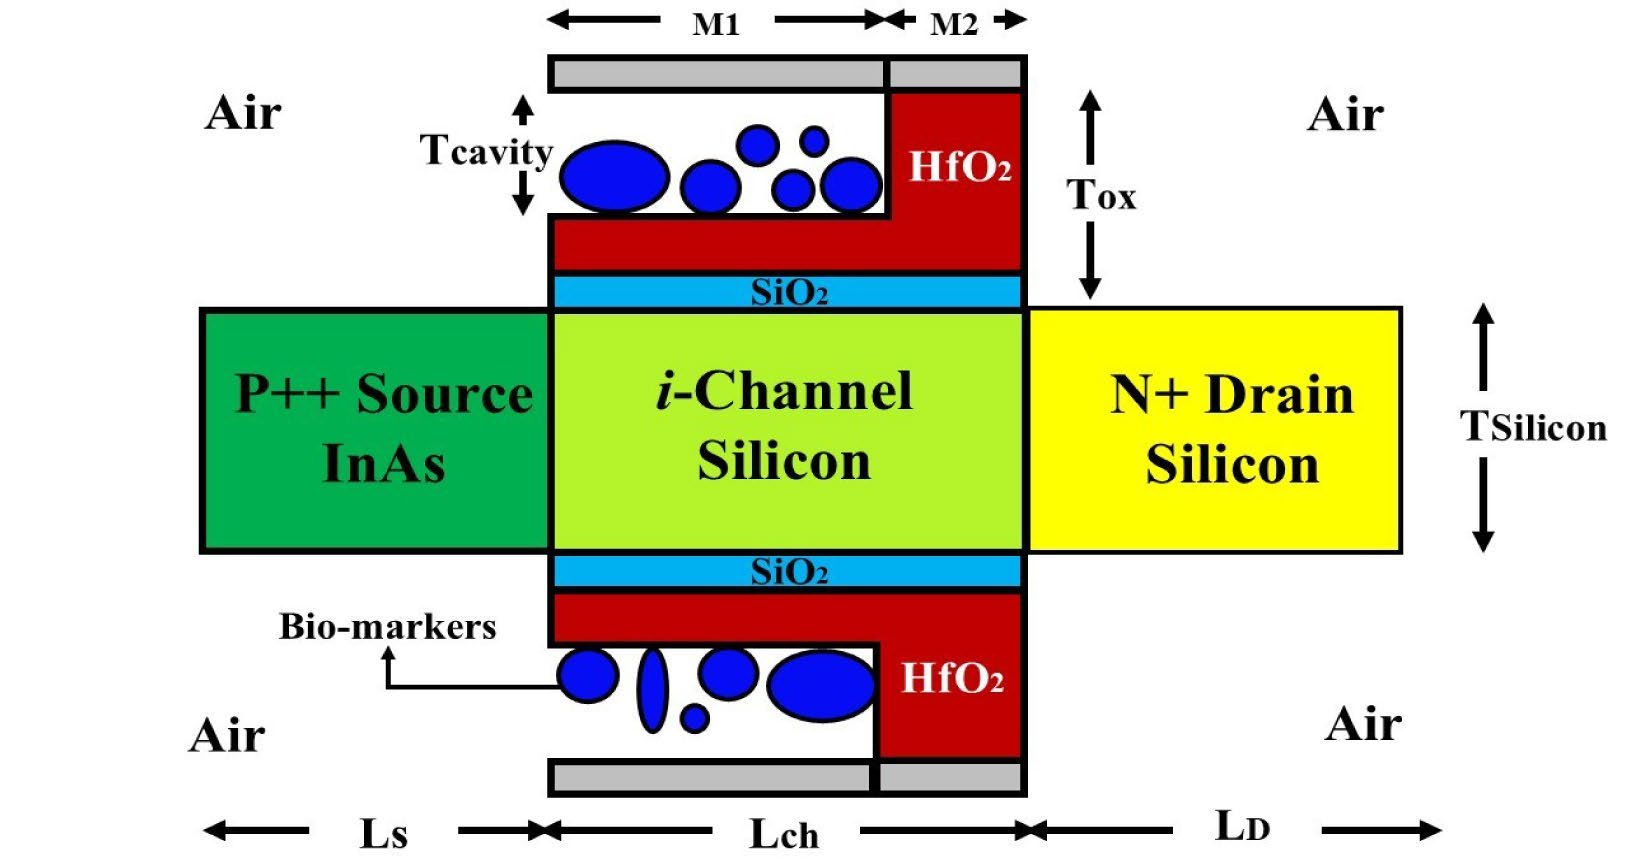
\includegraphics[width=0.85\columnwidth]{assets/images/faculty_psa_device.jpg}
    \captionof{figure}{Cross-section of the heterostructure oxide-engineered double-gate TFET biosensor.}
\end{minipage}
  \end{center}
\vspace{-0.35em}

  \subsection*{\centering\uppercase{Device and Simulation Model}}
  The structure is analysed with SILVACO ATLAS TCAD. Non-local BTBT, concentration- and field-dependent mobility, Fermi--Dirac statistics, Shockley--Read--Hall recombination, bandgap narrowing, trap-assisted tunnelling, and drift--diffusion transport are included. The transient Heiman model represents trap capture and emission during forward and reverse gate sweeps [1, 5].

  \noindent
  Calibration is performed against reported experimental characteristics of lateral p-type InAs--Si TFETs. Agreement is obtained using an interface-trap density of the order of $10^{12}\,\mathrm{cm}^{-2}$ at the Si--SiO$_2$ interface and a channel mobility near $590\,\mathrm{cm^2/(V\,s)}$. This calibration improves physical credibility, although it is not equivalent to fabricating and measuring the complete biosensor.

  \subsection*{\centering\uppercase{Fabrication Feasibility}}
  The proposed flow is informed by experimental lateral InAs--Si TFET integration using selective epitaxy and oxide templates [6]. A practical sequence would form the InAs source, silicon channel and drain, deposit the SiO$_2$/HfO$_2$ dielectric stack, define the dual-metal gate, etch the sensing cavities, and add a surface coating and linker chemistry for selective binding. Cavity etching and interface quality remain important fabrication risks because damage or roughness can increase the very traps examined in this work.
\end{multicols}

\begin{table}[tb]
\centering
\caption{Principal model dimensions and operating conditions.}
\small
  \setlength{\tabcolsep}{6pt}
  \renewcommand{\arraystretch}{1.3}
  \begin{tabular}{@{}>{\bfseries\RaggedRight\arraybackslash}p{0.28\textwidth}
                      >{\Centering\arraybackslash}p{0.20\textwidth}
                      >{\RaggedRight\arraybackslash}p{0.44\textwidth}@{}}
    \toprule
    \textbf{Parameter} & \textbf{Value} & \textbf{Purpose} \\
    \midrule
    Silicon body thickness & $10\,\mathrm{nm}$ & Nanoscale channel with double-gate control \\
    Oxide / cavity thickness & $11/8\,\mathrm{nm}$ & Gate stack and dielectric-modulation region \\
    Channel length & $40\,\mathrm{nm}$ & $30\,\mathrm{nm}$ M1 plus $10\,\mathrm{nm}$ M2 gate regions \\
    Source / drain doping & $10^{19}/5\times10^{18}\,\mathrm{cm}^{-3}$ & Degenerate p-type source and n-type drain \\
    Gate work functions & $3.8$ and $4.7\,\mathrm{eV}$ & Dual-material electrostatic engineering \\
    Gate / drain bias & $0$--$1.5\,\mathrm{V}$ / $1\,\mathrm{V}$ & Transfer sweep and readout condition \\
    Modelled interface traps & Up to $5\times10^{12}\,\mathrm{cm}^{-2}$ & Transient reliability and hysteresis analysis \\
    \bottomrule
  \end{tabular}
\end{table}
\vspace{-0.18em}

\begin{multicols}{2}
  \subsection*{\centering\uppercase{Fresh-Sensor Response}}
  Table~1 lists principal model dimensions and operating conditions.
  The electrostatic simulations show that increasing the cavity dielectric constant strengthens the electric field at the source--channel junction. For diseased-cell conditions, the tunnelling distance falls by roughly $70\%$ relative to the reference case, increasing BTBT rate and saturation drain current. The simulated switching ratio improves by several orders of magnitude, while the subthreshold slope becomes steeper for larger $\kappa$ values [1].

  \subsubsection*{Sensitivity Metrics}
  Drain-current sensitivity is defined relative to the air-filled cavity:
  \[
    S_{I_{\mathrm{ON}}}=\tfrac{I_{\mathrm{ON}}(\text{cell})}{I_{\mathrm{ON}}(\text{air})}.
  \]
  Subthreshold-slope sensitivity is
  \[
    S_{SS}=\tfrac{|SS(\text{cell})-SS(\text{air})|}{SS(\text{air})}.
  \]
  In the neutral-cell model, peak $S_{I_{\mathrm{ON}}}$ reaches approximately $1.11\times10^9$ for T47D at $V_G\approx1.05\,\mathrm{V}$. At a fixed $V_G=1.5\,\mathrm{V}$, T47D produces $S_{I_{\mathrm{ON}}}\approx7.77\times10^8$, while MCF-10A produces approximately $3.42\times10^5$. These large simulated differences motivate the use of drain current as a sensing signal.

  \noindent\begin{minipage}{\columnwidth}
  \subsubsection*{Effect of Fixed Cell Charge}
  Positive fixed charge near the cavity promotes inversion and shifts the transfer curve toward lower gate voltage; negative charge promotes accumulation and shifts it toward higher voltage. Fixed charge can therefore move the threshold and change sensitivity. The simulations distinguish this static shift from hysteresis: a fixed charge does not automatically create different forward and reverse curves.
  \end{minipage}

  \subsection*{\centering\uppercase{Trap-Induced Hysteresis}}
  Interface defects can capture electrons during an upward gate sweep and release them on a different timescale during the downward sweep. The resulting transfer curves no longer coincide.   Hysteresis width is measured at a chosen current criterion as
  \[
    HW=|V_{\mathrm{th,for}}-V_{\mathrm{th,rev}}|.
  \]
  A simplified dependence is
  \[
    HW\approx\tfrac{q f_t N_{it}}{C_{\mathrm{net}}},
  \]
  where $q$ is electronic charge, $f_t$ is trap occupancy, $N_{it}$ is interface-trap density, and $C_{\mathrm{net}}$ is the effective series capacitance.

  \begin{center}
\vspace{-0.5em}
\begin{minipage}{0.98\columnwidth}
\centering
    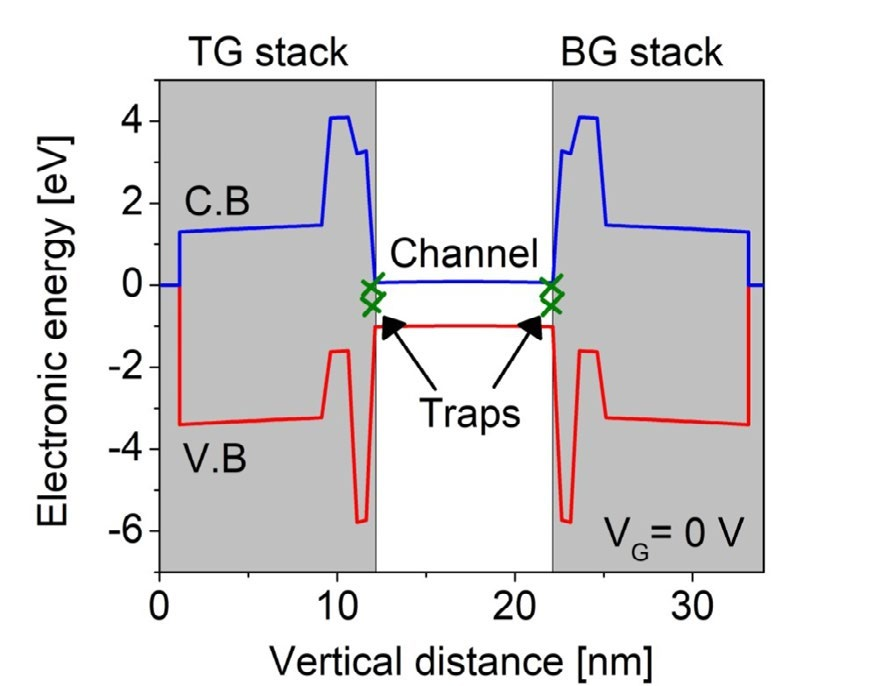
\includegraphics[width=0.82\columnwidth]{assets/images/faculty_psa_hysteresis.jpg}
    \captionof{figure}{Forward and reverse transfer curves defining hysteresis width for the T47D condition.}
\end{minipage}
  \end{center}
\vspace{-0.35em}

  \subsection*{\centering\uppercase{Sweep-Rate Dependence}}
  Sweep rate determines how long traps have to exchange charge with the channel. The study models a triangular gate waveform between $0$ and $1.5\,\mathrm{V}$. For T47D, hysteresis is approximately $10.2\,\mathrm{mV}$ at $1\,\mathrm{V/s}$, $16.3\,\mathrm{mV}$ at $0.1\,\mathrm{V/s}$, and $32.8\,\mathrm{mV}$ at $0.01\,\mathrm{V/s}$. A slow sweep allows more traps to capture and retain charge, increasing the difference between forward and reverse thresholds.

  \begin{center}
\vspace{-0.5em}
\begin{minipage}{0.98\columnwidth}
\centering
    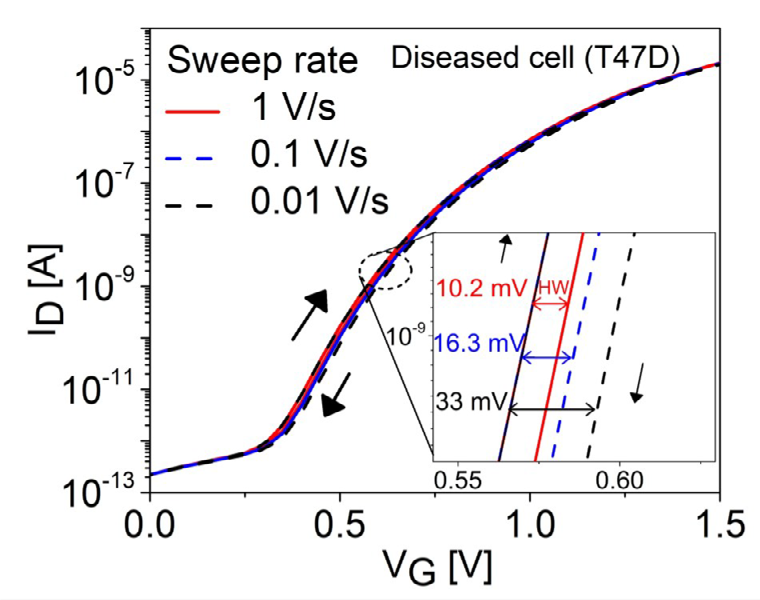
\includegraphics[width=0.84\columnwidth]{assets/images/faculty_psa_sweep_rate.png}
    \captionof{figure}{Simulated hysteresis increases as the gate sweep becomes slower.}
\end{minipage}
  \end{center}
\vspace{-0.35em}

  \subsection*{\centering\uppercase{Temperature and Trap Location}}
  At a fixed slow sweep rate, predicted hysteresis for the T47D condition rises from $32.8\,\mathrm{mV}$ at $300\,\mathrm{K}$ to $35.1\,\mathrm{mV}$ at $350\,\mathrm{K}$ and $40.2\,\mathrm{mV}$ at $400\,\mathrm{K}$. Higher temperature alters capture and emission times and increases thermal carrier velocity.

  \noindent
  Trap location also matters. The model compares defects at the crystalline InAs--Si heterojunction with those at the amorphous/crystalline Si--SiO$_2$ boundary. Across the investigated sweep rates, Si--SiO$_2$ traps produce larger hysteresis because their time-constant distribution interacts more strongly with the applied sweep. Reliability improvement therefore requires careful oxide growth, interface passivation, and low-damage cavity processing.

  \subsection*{\centering\uppercase{Damaged-Sensor Sensitivity}}
  Traps introduce recombination paths, reduce available channel carriers, and degrade on-current. The resulting drain-current sensitivity is lower than that of the fresh device for every modelled cell line. The study defines
  \[
    \text{Inaccuracy}=\left|
    \tfrac{S_{I_{\mathrm{ON}}}^{\mathrm{damaged}}-
    S_{I_{\mathrm{ON}}}^{\mathrm{fresh}}}
    {S_{I_{\mathrm{ON}}}^{\mathrm{fresh}}}
    \right|\times100\%.
  \]
  The predicted inaccuracy is about $97\%$ for MCF-10A, around $60\%$ for several intermediate diseased-cell conditions, and roughly $50\%$ for T47D. A sensor may therefore retain a seemingly large signal for a strongly coupled target while becoming unreliable near the healthy/disease decision boundary.

  \begin{center}
\vspace{-0.5em}
\begin{minipage}{0.98\columnwidth}
\centering
    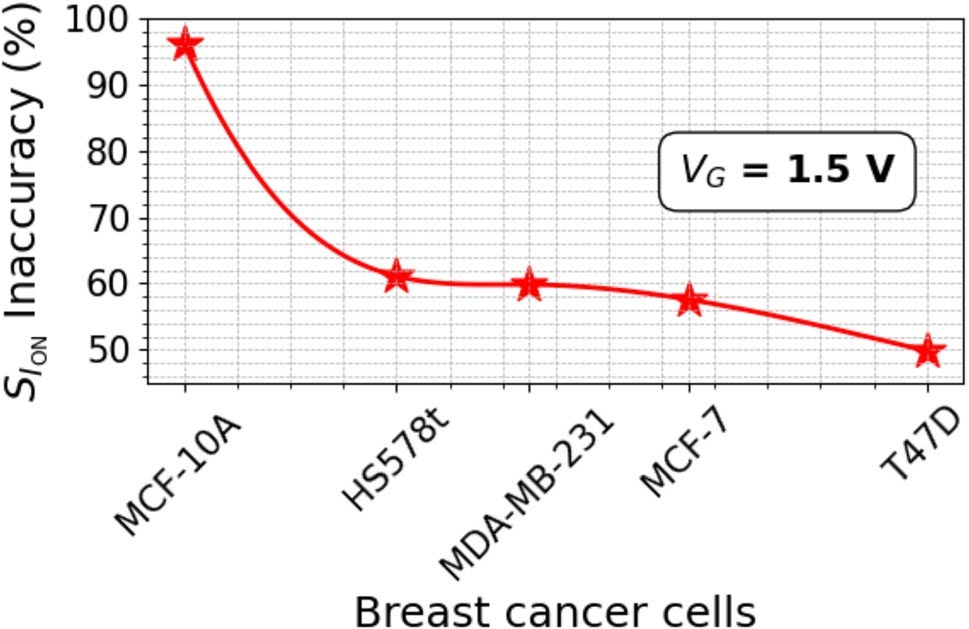
\includegraphics[width=0.85\columnwidth]{assets/images/faculty_psa_inaccuracy.jpg}
    \captionof{figure}{Sensitivity inaccuracy caused by trap degradation for the modelled cell conditions.}
\end{minipage}
  \end{center}
\end{multicols}

\begin{table}[t]
\centering
\caption{Key reliability results from the calibrated simulation study.}
\small
  \setlength{\tabcolsep}{6pt}
  \renewcommand{\arraystretch}{1.35}
  \begin{tabular}{@{}>{\bfseries\RaggedRight\arraybackslash}p{0.24\textwidth}
                      >{\Centering\arraybackslash}p{0.23\textwidth}
                      >{\RaggedRight\arraybackslash}p{0.45\textwidth}@{}}
    \toprule
    \textbf{Comparison} & \textbf{Predicted Result} & \textbf{Interpretation} \\
    \midrule
    T47D sweep rate: $1\rightarrow0.01\,\mathrm{V/s}$ & $HW:10.2\rightarrow32.8\,\mathrm{mV}$ & Slow measurement exposes more trap capture and delayed emission \\
    T47D temperature: $300\rightarrow400\,\mathrm{K}$ & $HW:32.8\rightarrow40.2\,\mathrm{mV}$ & Thermal activation increases trap participation \\
    Fixed positive cell charge, no switching traps & $HW\approx0$ & Static charge shifts threshold but does not create sweep-dependent hysteresis \\
    Si--SiO$_2$ versus InAs--Si traps & Larger $HW$ at Si--SiO$_2$ & Oxide-interface time constants dominate the simulated degradation \\
    MCF-10A fresh versus damaged sensitivity & Approximately $97\%$ inaccuracy & Reliability loss can hide or distort the healthy reference condition \\
    T47D fresh versus damaged sensitivity & $7.77\times10^8\rightarrow3.9\times10^8$ & Strong response remains, but absolute sensitivity is substantially reduced \\
    \bottomrule
  \end{tabular}
\end{table}
\vspace{-0.18em}

\begin{multicols}{2}
  \subsection*{\centering\uppercase{Sensitivity Versus Selectivity}}
  Table~2 summarizes key reliability results from the calibrated simulation study.
  Selectivity measures discrimination between the T47D target and other cell conditions. The damaged device can show a larger relative contrast for some comparisons even while its absolute current and sensitivity fall. This is not an improvement in overall sensing quality. A weak signal may appear relatively distinct yet remain difficult to measure accurately in the presence of noise, drift, device variability, and biological interference.

  \noindent
  Reliable benchmarking should therefore report the raw transfer curves, signal magnitude, sensitivity, selectivity, hysteresis, repeatability, noise, and calibration drift. Evaluating only one normalised metric can conceal device degradation.

  \subsection*{\centering\uppercase{Clinical and Experimental Limitations}}
  The reported results are calibrated TCAD predictions, not measurements from a fabricated H-OE-DG-TFET biosensor. No liquid-phase breast-cell assay is included. The assumed dielectric constants represent literature values and may vary with frequency, temperature, cell state, measurement method, surface coverage, and biological environment.

  \noindent
  A practical electrolyte creates an electric double layer and introduces biolayer capacitance, mobile ions, Debye screening, reference-electrode conditions, fluidic transport, non-specific adsorption, and surface-chemistry variability. These effects modify the effective capacitance and surface-potential coupling. Experimental work must also demonstrate selectivity through appropriate receptors and controls; dielectric contrast alone does not identify a cancer cell uniquely.

  \subsection*{\centering\uppercase{Design Guidance}}
  The study suggests several priorities for future devices:
  \begin{itemize}\justifying
    \item minimise Si--SiO$_2$ defect density through interface passivation and controlled processing;
    \item report gate sweep rate, direction, current criterion, temperature, and bias history with every hysteresis result;
    \item calibrate fresh and aged devices rather than assuming sensitivity remains constant;
    \item include liquid-gate electrostatics, receptor layers, ionic screening, and realistic biological noise;
    \item evaluate device-to-device variability and repeated measurement cycles;
    \item confirm the predicted response through fabrication and blinded biological testing.
  \end{itemize}

  \subsection*{\centering\uppercase{Conclusion}}
  The oxide-engineered InAs--Si double-gate TFET offers a promising simulated platform for dielectric-modulated breast-cancer sensing. Larger dielectric constants strengthen electrostatic coupling, shorten the tunnelling path, and increase drain-current sensitivity. The same device, however, is vulnerable to transient charge trapping at semiconductor interfaces.

  \noindent
  Trap-induced hysteresis depends strongly on measurement time and temperature, with the Si--SiO$_2$ interface producing the greatest degradation in the model. Sensitivity loss can be severe even when selectivity appears acceptable. The central lesson is that a biosensor cannot be judged by peak sensitivity alone: stability, hysteresis, inaccuracy, fabrication quality, measurement protocol, and experimental validation must be designed together.

  \subsection*{\centering\uppercase{References}}
  {\small
  \begin{justify}
    \begin{enumerate}[label={\relax[\arabic*]},leftmargin=*,labelsep=0.5em,itemsep=0.20em,parsep=0pt]
      \item R. Ghosh and P. Saha, “Modeling trap dynamics in oxide-engineered heterostructure TFETs for breast cancer detection,” \textit{Scientific Reports}, vol. 16, art. 3970, 2026.
      \item H. Im et al., “A dielectric-modulated field-effect transistor for biosensing,” \textit{Nature Nanotechnology}, vol. 2, no. 7, pp. 430--434, 2007.
      \item S. Shreya et al., “Core-shell junctionless nanotube tunnel field effect transistor: Design and sensitivity analysis for biosensing application,” \textit{IEEE Sensors Journal}, vol. 20, no. 2, pp. 672--679, 2020.
      \item M. Hussein et al., “Breast cancer cells exhibit specific dielectric signatures in vitro,” \textit{Scientific Reports}, vol. 9, art. 4681, 2019.
      \item F. Heiman and G. Warfield, “The effects of oxide traps on the MOS capacitance,” \textit{IEEE Transactions on Electron Devices}, vol. 12, no. 4, pp. 167--178, 1965.
      \item K. E. Moselund et al., “Lateral InAs/Si P-type tunnel FETs integrated on Si---Part 1: Experimental devices,” \textit{IEEE Transactions on Electron Devices}, vol. 63, no. 11, pp. 4233--4239, 2016.
      \item S. Sant et al., “Lateral InAs/Si P-type tunnel FETs integrated on Si---Part 2: Simulation study of the impact of interface traps,” \textit{IEEE Transactions on Electron Devices}, vol. 63, no. 11, pp. 4240--4247, 2016.
      \item R. Ghosh et al., “Theoretical insights into the impact of border and interface traps on hysteresis in monolayer MoS$_2$ FETs,” \textit{Microelectronic Engineering}, vol. 299, art. 112333, 2025.
      \item Silvaco, \textit{ATLAS User's Manual}, Santa Clara, CA, USA.
    \end{enumerate}
    \end{justify}}
\end{multicols}